\section{Amplitude-Attenuated Datasets}
\label{sec:seq}
There are a number of \ac{NMR} experiments in which the
variation of a particular pulse sequence parameter over a number of iterations
leads to the generation of a series of
\acp{FID} with the same form except for discrepancies in their amplitudes.
In this section, an extension of the established \ac{1D} estimation
technique is described, facilitating the analysis of datasets acquired using
these experiments.
After the most prominent examples of the relevant experiments are
introduced, the methodology of the estimation method is described.
Finally, its performance when applied to both simulated and experimental
datasets is showcased.

\subsection{Relaxation Experiments}
\label{subsec:relaxation_experiments}
Any spin system which has been perturbed from its equilibrium position will
eventually return to equilibrium due to relaxation. As introduced in
\cref{chap:intro}, the simplest model of relaxation centers around two
processes: longitudinal relaxation and transverse relaxation, whose rates are
quantified by the times $T_1$ and  $T_2$ respectively.
Numerous factors affect these times  including the rate at which the spin
tumbles in space, and its electronic environment.
The $T_1$ and $T_2$ values of the spins in a sample provide valuable insight
into the chemical system being studied, and can also help to guide
spectroscopists in the determination of optimal pulse sequence
parameters\footnote{
    For example, after a pulse sequence has been run, it is necessary to include a
    delay (called the \emph{relaxation delay}) prior to
    re-running it, to enable the spin system's longitudinal magnetisation to
    sufficiently recover. Having an understanding of the $T_1$ values
    associated with a sample can help to determine a relaxation delay which is
    long enough to facilitate sufficient recovery, but that is not overly long, to
    avoid an experiment time which is longer than necessary.
}.

\subsubsection{Measuring $T_1$: Inversion Recovery}
\label{subsec:invrec}
The inversion recovery experiment involves the simple pulse sequence $\ang{180}
\rightarrow \tau \rightarrow \ang{90} \rightarrow \tone$, where $\tone$ is the
period during which \ac{FID} acquisition takes place. The initial
\ang{180} pulse inverts the magnetisation, so that it is along $-z$ in the
context of the Bloch model. During $\tau$, the spin system undergoes longitudinal
relaxation, with the spin state populations gradually being driven back to
their equilibrium configuration. The \ang{90} pulse rotates the magnetisation
into the transverse plane, enabling detection. The resultant phase and
magnitude of each signal is directly related to the amount of time that
longitudinal relaxation is allowed to occur. With $\tau = \qty{0}{\second}$,
signals with maximal amplitude, but phases of \ang{180} (equivalent to a
negative amplitude) will result. At the other extreme of $\tau \gg T_1$,
the spin system will have reverted
back to equilibrium, such that the signals will also have maximal amplitudes,
but phases of \ang{0}. By sequentially adjusting $\tau$ in a
\ac{2D} experiment, a series of \acp{FID} will be obtained in which the intensity
of a given signal, arising from a spin with longitudinal time $T_1$, will vary
according to
\begin{equation}
    a\left(\tau\right) = a_{\infty} \left( 1 - 2 \exp\left( -\frac{\tau}{T_1}\right) \right),
\end{equation}
where $a_{\infty}$ is the intensity of the signal when the spin system
has returned to equilibrium. Note that $a(0) = -a_{\infty}$, as the magnetisation
has been completely inverted, and no time has been allowed for longitudinal
relaxation to take place. An example of a series of spectra acquired using a
(simulated) inversion recovery experiment is given by
\cref{fig:five-multiplets-invrec}.d.

\subsubsection{Measuring $T_2$: \acs{CPMG}}
\label{subsec:cpmg}
Inspired by the inversion recovery experiment, one might assume
that the pulse sequence $\ang{90} \rightarrow \tau \rightarrow \tone$ would be
effective for  $T_2$ determination. However the effects of J-modulation would
generate undesirable spectra with phase-modulated peaks. As well as this the
presence of field inhomogeneities will cause relaxation at a faster rate than
anticipated; the effect of field inhomogeneities is incorporated into the
``observed'' transverse relaxation time, $T_2^* < T_2^{\vphantom{*}}$\footnote{
    $T_2^*$ is defined by the expression
    $\nicefrac{1}{T_2^*} \coloneq \nicefrac{1}{T_2} + \gamma \Updelta B_0$,
    where $\Updelta B_0$ is the variation in magnetic field strength across the
    sample volume.
    \label{fn:t2-star}
}\cite{Chavhan2009}. The effects of
J-modulation and field inhomogeneity can be nullified if rapid refocussing is
applied, by subjecting the spin system to a train of spin echoes. The classic
route to $T_2$ measurement is the \ac{CPMG}
experiment\cite{Carr1954,Meiboom1958}, comprising $\ang{90}_x \rightarrow
\left[ \tau \rightarrow \ang{180}_y \rightarrow \tau \right]_n \rightarrow
\tone$, where the spin echo duration $\tau$ is short and fixed, and the number
of cycles $n$ can be varied to alter the total evolution time. The number of
\ac{CPMG} cycles applied affects the intensity of the resulting signal
according to
\begin{equation}
    a(n) = a_0 \exp\left(-\frac{2 \tau n}{T_2}\right),
\end{equation}
where $a_0$ is the intensity where no spin echo cycles were employed, such that
the pulse sequence is reduced to the standard pulse-acquire experiment. Recent
enhancements to the \ac{CPMG} approach, including the \ac{PROJECT} pulse
sequence\cite{Aguilar2012} are also well-suited to $T_2$ determination.

\subsection{Diffusion Experiments}
\label{subsec:diffusion_experiments}
\ac{NMR} is well established as a means of determining the rates of
translational diffusion of chemical species\cite{Johnson1999,Morris2009b}.
The rate of translation of a species is given by the translational
diffusion coefficient, $D$ (\unit{\meter\squared\per\second})\cite[Chapter
19]{Atkins2014}.
The first illustration of the determination of the diffusion coefficient using
\ac{NMR} came from Stejskal and Tanner, in which they described the \ac{PGSE}
pulse sequence\cite{Stejskal1965} (\cref{fig:diffusion_sequences}.a).
The \ac{PGSE} sequence consists of a conventional spin-echo ($\ang{90}_x
\xrightarrow{\tau} \ang{180}_y \xrightarrow{\tau} \text{acquire}$), with
\acp{PFG} applied after each of the \ac{RF} pulses.
As a simple overview of how the pulse sequence works, consider a single spin on
resonance with the transmitter (i.e. its rotating frame frequency is zero) in a
sample tube at position $z \in [-\nicefrac{l_z}{2}, \nicefrac{l_z}{2}]$ along
the main field axis, where $l_z$ is the length of the sample lying within the
receiver coil (typically about $\qty{1.5}{\centi\meter}$).
After the \ang{90} pulse, the magnetisation will be $-M_y$.
During the first \ac{PFG}, the spin's resonance frequency will become
$\omega_{\text{PFG}} = -\gamma g z$, where $g$ is the strength of the \ac{PFG}
(\unit{\tesla\per\meter})\footnote{
    Gradient strengths are often expressed in the non-\ac{SI} units of
    \unit{\gauss\per\centi\meter}, which is equivalent to
    \qty[print-unity-mantissa = false]{e-2}{\tesla\per\meter}.
}.
Assuming the gradient is applied for a time $\delta$, the spin will
precess by the angle $\alpha = -\gamma g z \delta$. After the \ang{180}
pulse, the spin's magnetisation will be as follows:
\[
    -M_y
    \xrightarrow{\text{PFG}} -M_y \cos(\alpha) + M_x \sin(\alpha)
    \xrightarrow{\ang{180}_y} -M_y \cos(\alpha) - M_x \sin(\alpha).
\]
Suppose the spin has moved to a new position $z + \Updelta_z$
between the end of the first gradient and the beginning of the second.
Application of the second gradient will cause precession by the angle
$\beta = -\gamma g (z + \Updelta_z) \delta$:
\begin{equation*}
   \begin{split}
        \xrightarrow{\text{PFG}}
            &-M_y \cos(\alpha)\cos(\beta) +
            M_x \cos(\alpha)\sin(\beta) -
            M_x \sin(\alpha)\cos(\beta) -
            M_y \sin(\alpha)\sin(\beta)\\
        &= -M_y \cos(\gamma g \delta \Updelta_z) -
           M_x \sin(\gamma g \delta \Updelta_z),
   \end{split}
\end{equation*}
The \acp{PFG} have been been employed to encode the change in
$z$-coordinate of the spin after a known amount of time, by influencing the
phase of the magnetisation relative to its phase immediately after the \ang{90}
pulse.
Extending this idea to a system of many identical spins, which will translate
by different extents between the \acp{PFG}, individual spin contributions to
the bulk magnetisation will become dephased, leading to an attenuation of the
amplitude of the resulting \ac{FID}. For species which diffuse at a faster
rate, the dephasing effect is more severe, such that a more rapid attenuation
results for a given increase in $g$.

\begin{figure}
   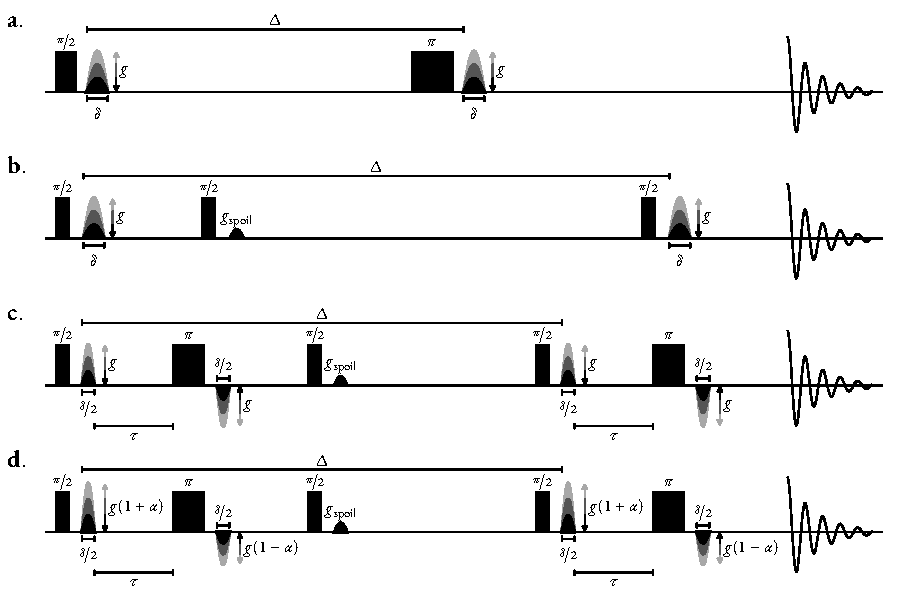
\includegraphics{diffusion_sequences/diffusion_sequences.pdf}
   \caption[
       Pulse sequences used for the determination of translational diffusion constants.
   ]{
       Pulse sequences used for the determination of translational diffusion constants.
       \textbf{a.} \acs{PGSE},
       \textbf{b.} \acs{PGSTE},
       \textbf{c.} \acs{PGSTEBP},
       \textbf{d.} One-shot DOSY.
       \ac{RF} pulses are denoted by solid rectangles. Diffusion-encoding
       gradients are denoted by sine-bell shapes with varying shades,
       indicating that the intensity ($g$) is incremented to create a \ac{2D}
       dataset. Spoiler gradients are denoted by solid black sine-bell shapes.
   }
   \label{fig:diffusion_sequences}
\end{figure}

Through consideration of the Bloch-Torrey equations\cite{Torrey1956}, which
extend the classic Bloch equations to account for the effects of diffusion on
magnetisation, the following equation, known as the \emph{Stejskal-Tanner
equation}, may be derived:
\begin{equation}
    a(g) = a_0 \exp \left(- \gamma^2 \delta^2 g^2 D \left(\Updelta -
    \frac{\delta}{3}\right)\right),
    \label{eq:stejskal_tanner}
\end{equation}
where
$a_0$ is the amplitude of a given signal without the application of \acp{PFG},
$\delta$ is the duration of each \ac{PFG} (\unit{\second}), and
$\Updelta$ is the delay between the \acp{PFG}, often known as the \emph{diffusion time}
(\unit{\second}),
While \cref{eq:stejskal_tanner} is widely stated in the diffusion \ac{NMR}
literature, it is only strictly applicable when the \ac{PGSE} sequence is used,
and \acp{PFG} with rectangular amplitude profiles are applied\footnote{
    Rectangular \acp{PFG} (i.e. those in which there is an infinitesimal time
    to rise to full strength, and to fall back to zero) are technically
    impossible to achieve as they would require gradient coils with zero
    inductance, though in practice it is possible to generate gradients with
    behaviour close to this.
}. As will be discussed soon, the exact form of the pulse sequence impacts the
functional form by which $a(g)$ varies.

Tanner introduced a variant of the original \ac{PGSE} experiment called
\ac{PGSTE}\cite{Tanner1970} (\cref{fig:diffusion_sequences}.b). Instead
of the diffusion period being bisected by a
\ang{180} pulse, \ac{PGSTE} features two \ang{90} pulses at the beginning and
end of the diffusion period.
Hence, the extent of signal loss due to relaxation is affected by $T_1$ in
\ac{PGSTE}, as opposed to $T_2$ in \ac{PGSE}. \ac{PGSTE} is therefore favoured
in scenarios where $T_1 \ll T_2$, as improved data sensitivity is achievable.

Both \ac{PGSE} and \ac{PGSTE} employ \emph{monopolar} \acp{PFG} for diffusion
encoding.
Experiments also exist which employ
\emph{bipolar} gradient elements, which consist of a
\ac{PFG}, followed by a \ang{180} pulse, and then a second \ac{PFG} with the
opposite polarity to the first\cite{Cotts1989,Wu1995}. The \ac{PGSTEBP} experiment
(\cref{fig:diffusion_sequences}.c) can be thought of as the bipolar analogue of
\ac{PGSTE}.
Bipolar gradients are useful in circumstances where it is important to purge
the effects of static gradients in the sample, caused by field inhomogeneities.
Morris and coworkers have developed the \emph{one-shot}
experiment\cite{Pelta2002} (\cref{fig:diffusion_sequences}.d), which requires a
single transient per gradient strength (i.e. there is no requirement for a
phase-cycling scheme).  This is achieved through the use of bipolar gradients
which comprise asymmetrical \acp{PFG} with relative powers $1 + \alpha : 1 -
\alpha$ for some $ 0 > \alpha > 1$ (commonly, $\alpha=0.2$).

The most common means of conducting a diffusion experiment is to run one of
pulse sequences mentioned above (or variants thereof) with $g$ varied across
increments.
It is virtually always the case that the \ac{FID}'s signal amplitudes will
abide by the following general form of the Stejskal-Tanner equation,
regardless of the exact pulse sequence used:
\begin{equation}
    a(g) = a_0 \exp\left(- c g^2 D\right),
\end{equation}
for some constant $c$ (\unit{\tesla\per\second\squared}).
The functional form of $c$ depends on the type of experiment used, as well as
the amplitude profile (\emph{shape}) of the \acp{PFG}.
A consideration of the Bloch-Torrey equations for a given experiment is
necessary, with an extensive overview provided by Sinnaeve for most diffusion
NMR experiments\cite{Sinnaeve2012}. In general, $c$ is as follows:
\begin{equation}
    c = \gamma^2 \delta^2 \sigma^2 \Updelta^{\prime}.
    \label{eq:stejskal_tanner_generic}
\end{equation}
$\sigma$ is the \emph{shape factor} of the \acp{PFG} (\textit{vide infra}),
and $\Updelta^{\prime}$ is the effective time that diffusion is allowed
to occur. Examples of the form that $\Updelta^{\prime}$ takes include:
\begin{equation}
    \Updelta^{\prime} =
    \begin{cases}
        \Updelta + 2 \left(\kappa - \lambda\right) \delta &
        \text{\ac{PGSE}, \ac{PGSTE}}\\
        \Updelta + \frac{\left(2 \kappa - 2 \lambda - 1\right)\delta}{4} - \frac{\tau}{2} &
        \text{\ac{PGSTEBP}} \\
        \Updelta + \frac{\left(\kappa - \lambda\right)
            \left(\alpha^2 + 1\right) \delta}{2} +
        \frac{\left(\delta + 2 \tau\right)\left(\alpha^2 - 1\right)}{4} &
        \text{One-shot}
    \end{cases}.
    \label{eq:Delta-prime}
\end{equation}
$\tau$ is the delay between the initial \ac{PFG} and the \ang{180} pulse in
experiments with bipolar gradients.
The factors $\sigma$,  $\lambda$, and $\kappa$ are related to the shape
function $s(\epsilon) : \epsilon \in [0, 1]$ of the \ac{PFG}, which describes
the variation of the gradient amplitude as a function of its progression.
For a rectangular gradient, $s(\epsilon) = 1 \forall \epsilon$, whereas for a
sine-bell gradient, $s(\epsilon) = \sin(\pi \epsilon)$. The cumulative
distribution of the shape function is given by:
\begin{equation}
    S(\epsilon) = \int_0^{\epsilon} s\left(\epsilon^{\prime}\right)
            \mathrm{d} \epsilon^{\prime} \quad \forall \epsilon \in [0, 1].
\end{equation}
The corresponding definition of $S$ for the case of a gradient made of $N$
discrete steps with shape $\symbf{s} \in \mathbb{R}^{N}$ is
\begin{equation}
    S_n =
        \frac{1}{n} \sum_{i = 1}^{n} s_i \quad
        \forall n \in \left\lbrace 1, \cdots, N\right\rbrace,
\end{equation}
$\sigma$, $\lambda$, and $\kappa$ are related to the shape function's
cumulative distribution as follows:
\begin{subequations}
    \begin{gather}
        \sigma = S(1),\\
        \lambda = \frac{1}{\sigma} \int_0^1 S(\epsilon) \mathrm{d} \epsilon,\\
        \kappa = \frac{1}{\sigma^2} \int_0^1 S^2(\epsilon) \mathrm{d} \epsilon,
    \end{gather}
\end{subequations}
with their discrete counterparts being:
\begin{subequations}
    \begin{gather}
        \sigma = S_{N} \\
        \lambda = \frac{1}{\sigma N} \sum_{n = 1}^{N} S_n
            = \frac{1}{\sigma N} \sum_{n=1}^{N}
            \left(\frac{1}{n} \sum_{i=1}^{n} s_i\right) \\
        \kappa = \frac{1}{\sigma^2 N} \sum_{n = 1}^{N} S^2_n
            = \frac{1}{\sigma^2 N} \sum_{n = 1}^{N}
            \left(\frac{1}{n} \sum_{i=1}^{n} s_i\right)^2.
    \end{gather}
\end{subequations}
For \acp{PFG} with a symmetrical shape, $\lambda = \nicefrac{1}{2}$. $\kappa$
is typically equal to or close to $\nicefrac{1}{3}$. It can now be seen that
the original Stejskal-Tanner equation for the
\ac{PGSE} experiment (\cref{eq:stejskal_tanner}) comes from
inserting \cref{eq:Delta-prime} into \cref{eq:stejskal_tanner_generic},
assuming a rectangular shape factor for the \acs{PFG}:
$\sigma = 1$,  $\lambda = \nicefrac{1}{2}$, and  $\kappa = \frac{1}{3}$.
In many situations,  $\Updelta$
dominates in the expression of $\Updelta^{\prime}$, and so ensuring the correct
form of $c$ could be seen as excessive. However, especially when  $\Updelta$ is
not orders of magnitude greater than $\delta$, the exact form of
$\Updelta^{\prime}$ used in \cref{eq:stejskal_tanner_generic} will be
important for accurate measurements of the diffusion coefficient.

\subsection{Analysing the Datasets}
Determining the quantity of interest from the above experiments is most
typically done using the following procedure:
\begin{enumerate}
    \item The series of \acp{FID} are processed in an equivalent fashion,
        leading to a set of \ac{1D} spectra.
    \item Peak-picking is performed to locate the chemical shift values which
        correspond to signals of interest within the spectra.
    \item For each chemical shift of interest, the values of the spectra are
        extracted, and the relevant function (see
        \cref{tab:seq-equations}) is fit to these values.
\end{enumerate}
This method is \emph{univariate} in the sense that it considers a single sample
(chemical shift) in isolation from the rest of the data.
It is popular to visualise the result of univariate fitting by plotting \ac{2D}
pseudo-spectra, featuring axes denoting (a) chemical shift, and (b)
the parameter of interest. Distributions taking
into account the predicted value of interest and the associated uncertainty
are plotted at each chemical shift.
In the context of diffusion \ac{NMR}, this form of data analysis is
referred to as \ac{DOSY}\cite{Morris2009b}.
The \ac{DOSY} approach works well in cases where peaks of interest are intense
and well-resolved. However, when there is considerable peak overlap, accurately
determining the parameter of interest associated with a given signal becomes
more challenging, since nearby signals will influence the rate of amplitude
decay. An aggregated value of the decay rates of the contributing signals
will be predicted using the above approach.
In such cases, it is possible to instead fit
a superposition of functions to the spectral amplitudes, as a means of
separating out contributions from the overlapping signals\cite{Nilsson2006}.
However, this process is usually only effective when the data has very high
\ac{SNR}, and the quantities of interest associated with the overlapping
signals differ considerably.

An alternative approach
is to use a \emph{multivariate} analysis method, which considers the entire
spectrum holistically, and attempts to decompose the spectrum into components
with different decay rates. Prominent examples of multivariate methods
developed for diffusion data analysis are \ac{DECRA}\cite{Windig1998} and
\emph{speedy} component resolution (\acs{SCORE})\cite{Nilsson2008}, an
improvement of the original \acs{CORE}\cite{Stilbs1996,Stilbs1996b}.
\acused{SCORE}\acused{CORE}
Multivariate techniques tend to only be only effective in situations where a
few (2 or 3) different signal decay rates are present. In diffusion
\ac{NMR}, each molecule in the sample will give rise to the same decay rate
across its signals (effects such as chemical exchange can lead to exceptions to
this: \cref{fig:andrographolide-dosy} provides an example of this).
These methods are generally unsuitable for inversion recovery and \ac{CPMG} datasets:
each spin in a sample will possess different $T_1$ and $T_2$ values, such that
a far greater number of decay rates will be present.

\subsection{Methodology}
A straightforward extension of \ac{1D} parametric estimation
provides a route to estimating amplitude-attenuated datasets in a
fashion with similarities to the traditional univariate (\ac{DOSY}) approach.
In this section, the theory of this method is discussed.

The datasets of interest can be considered in a general fashion.
Suppose the experiment is run with $K \in \mathbb{N}$ increments,
such that there is a vector  $\symbf{p} \in \mathbb{R}^K$ comprising the
values of the pulse sequence variable used to acquire each \ac{1D} \ac{FID} in
the data.  The complete dataset is expected to take the form $\symbf{Y} \in
\mathbb{C}^{K \times N}$ in which the value of the pulse sequence variable
affects the amplitudes of the contributing signals:
\begin{equation}
    \begin{gathered}
        y_{k,n} = \sum_{m=1}^{M} a_{k,m} \exp(\iu \phi_m)
        \exp((2 \pi \iu (f_m - \foff) - \eta_m) n \Dt),\\
        \forall k \in \lbrace 1, \cdots, K \rbrace,\ \forall n \in \lbrace 0,
        \cdots, N-1 \rbrace.
    \end{gathered}
\end{equation}
$\symbf{A} \in \mathbb{R}^{K \times M}$ is a matrix of the signal amplitudes
across the \acp{FID}:
\begin{equation}
    \symbf{A} =
    \begin{bmatrix}
        a_{1,1} & a_{1,2} & \cdots & a_{1,M}\\
        a_{2,1} & a_{2,2} & \cdots & a_{2,M}\\
        \vdots & \vdots & \ddots & \vdots\\
        a_{K,1} & a_{K,2} & \cdots & a_{K,M}
    \end{bmatrix}
\end{equation}
A complete parameter vector for the dataset is given by $\bth \in
\mathbb{R}^{(K + 3)M}$:
\begin{equation}
    \bth =
    \begin{bmatrix}
        \symbf{a}_1 & \cdots & \symbf{a}_K & \bdphi\T & \bdf\T & \bdeta\T
    \end{bmatrix}\T,
\end{equation}
where $\symbf{a}_k \in \mathbb{R}^M$ denotes the relevant row in $\symbf{A}$.
The amplitudes are a function of the pulse sequence variable with the following
form:
\begin{equation}
    a_{k,m} = a_{0,m} \mathcal{A} (\psi_m \hspace*{2pt} | \hspace*{2pt} p_k).
\end{equation}
$\symbf{a}_0 \in \mathbb{R}^{M}$ is a vector of the ``maximal
amplitudes'' of the signals, and $\symbf{\psi} \in \mathbb{R}^M$ is a vector
of the parameter of interest ($T_1$,  $T_2$, $D$) associated with
each signal. $a_{0,m}$ can be thought of as the largest
possible amplitude that could be obtained for signal $m$ with the given
pulse sequence:
\begin{itemize}
    \item In an inversion recovery experiment, the largest amplitude is
        achieved as $\tau \rightarrow \infty$, as the spin system will have
        returned back to equilibrium prior to the \ang{90} pulse.
    \item With \ac{CPMG} experiments, the largest amplitude will occur when
        $n = 0$, as no time is designated for transverse
        relaxation to take place.
    \item For diffusion experiments, the largest amplitude is achieved when
        $g=0$, since no diffusion-induced dephasing of spins will have
        occurred.
\end{itemize}
The function $\mathcal{A}$ describes how the amplitudes of resonances are
attenuated by the experimental variable, and has a form which is intimately
linked to the type of experiment. For the experiments described in
\cref{subsec:relaxation_experiments,subsec:diffusion_experiments},
the forms of $\mathcal{A}$ are listed in \cref{tab:seq-equations}.
\begin{table}
    \begin{center}
        \begin{tabular}{ccccccc}
            \hline
            Experiment &
            $p$ &
            $\psi$ &
            $\mathcal{A}(\psi | p)$ &
            $\frac{\partial \mathcal{A}(\psi | p)}{\partial \psi}$ &
            $\frac{\partial^2 \mathcal{A}(\psi | p)}{\partial \psi^2}$ \\ \hline
            Inv. Recov.&
            $\tau$ &
            $T_1$ &
            $\left(1 - 2 \exp \left(-\frac{\tau}{T_{1}}\right)\right)$ &
            $-\frac{2 \tau}{T_1^2} \exp\left(-\frac{\tau}{T_1}\right)$ &
            $\frac{2 \tau}{T_1^3} \exp\left(-\frac{\tau}{T_1}\right)\left(2 - \frac{\tau}{T_1}\right)$\\
            \acs{CPMG} &
            $n$ &
            $T_2$ &
            $\exp\left(-\frac{2 \tau n}{T_2}\right)$ &
            $\frac{2 \tau n}{T_2^2}\exp\left(-\frac{2 \tau n}{T_2}\right)$ &
            $\frac{2 \tau n}{T_2^3}\exp\left(-\frac{2 \tau n}{T_2}\right)
            \left( \frac{2 \tau n}{T_2} - 2 \right)$ \\
            Diffusion &
            $g$ &
            $D$ &
            $\exp\left(-c g^2 D\right)$ &
            $-c g^2 \exp\left(-c g^2 D\right)$ &
            $c^2 g^4 \exp\left(-c g^2 D\right)$ \\
            \hline
       \end{tabular}
       \caption[
           The various functional forms of $\mathcal{A}$ according to the
           different amplitude-attenuating NMR experiments considered.
       ]
       {
           The various functional forms of $\mathcal{A}$ according to the
           different amplitude-attenuating NMR experiments considered, along
           with its first and second derivatives, which are required to extract
           estimates of $\psi$ using \ac{NLP}.
       }
       \label{tab:seq-equations}
    \end{center}
\end{table}

\subsubsection{Estimating the Datasets}
The close relationship between the \acp{FID} within the dataset means that
completely estimating all of them separately, without exploiting information
from previously estimated \acp{FID}, is unnecessary.
Instead, after the first increment is estimated without prior knowledge,
yielding $\bth_{k=1} \in \mathbb{R}^{4M}$, the phases, frequencies and damping
factors, all of which are anticipated to remain the same across the
\acp{FID}, are fixed.
Subsequent parameter estimates are determined by taking the result from
the previous \ac{FID}, and subjecting it to \iac{NLP} routine in which only
the amplitudes are optimised. Thus, estimating each subsequent iteration
is reduced to the problem\footnote{
    $\mathcal{F}$ in \cref{eq:fidelity-amp} reads as ``the fidelity
    with respect to the amplitudes $\bda$, given phases $\bdphi_{k=1}$,
    frequencies $\bdf_{k=1}$, damping factors  $\bdeta_{k=1}$, and \ac{FID}
    $\by_k$''. The fidelity has exactly the same mathematical form as
    \cref{eq:fidelity}, though it has been emphasised that the phases,
    frequencies and damping factors are no longer variables to be optimised,
    but fixed parameters.
}
\begin{equation}
    \symbf{a}_k = \argmin_{\bda \in \mathbb{R}^M}
        \mathcal{F}(\bda \hspace*{2pt} | \hspace*{2pt}
        \bdphi_{k=1}, \bdf_{k=1}, \bdeta_{k=1}, \by_k)\quad\forall k \in \lbrace2, \cdots, K\rbrace.
        \label{eq:fidelity-amp}
\end{equation}
\Iac{NLP} routine can solve this very efficiently, typically in a few
iterations, on account of the linear dependence of the model with respect to
the oscillator amplitudes. The linear dependence means that second
derivatives of the model are all zero (see \cref{eq:amp-second-deriv}),
such that only first derivatives need to be computed to derive an exact Hessian
matrix of the fidelity.
Due to the linear dependence on amplitudes, an alternative means of
deriving amplitudes for each increment is to compute the following:
\begin{subequations}
    \begin{gather}
        \symbf{a}_k = \symbf{Z}^+ \symbf{y}_k, \\
        \symbf{Z} =
        \begin{bmatrix}
            1 & \cdots & 1 \\
            z_1 & \cdots & z_M\\
            \vdots & \ddots & \vdots \\
            z_1^{N-1} & \cdots & z_M^{N-1}
        \end{bmatrix}
        \begin{bmatrix}
            \exp(\iu \phi_1) \\ \vdots \\ \exp(\iu \phi_M)
        \end{bmatrix},\\
        z_m = \exp((2\pi \iu (f_m - \foff) - \eta_m)\Dt).
    \end{gather}
\end{subequations}
An outline of the estimation procedure is provided by \cref{alg:estimate-seq}.

\begin{algorithm}
    \caption[
        The proposed routine for estimating a sequence of amplitude-attenuated
        \acsp{FID}.
    ]
    {
        The proposed routine for estimating a sequence of amplitude-attenuated
        \acsp{FID}.
        \textsc{NLPAmp} denotes a
        routine which is akin to \textsc{NLP} (\cref{alg:nlp}), except
        only amplitudes are optimised; phases, frequencies and damping factors
        are fixed.
    }
    \label{alg:estimate-seq}
    \begin{algorithmic}[1]
        \Procedure{EstimateAmpAttenuated}{
            $\bY \in \mathbb{C}^{K \times N},
            \symbf{r}_{\text{interest}} \in \mathbb{R}^2,
            \symbf{r}_{\text{noise}} \in \mathbb{R}^2,
            M \in \mathbb{N}_0$
        }
        \State $\bth_{1}, \symbf{\epsilon}_{1} \gets \textsc{Estimate$1$D}\left(
            \by_1, \symbf{r}_{\text{interest}}, \symbf{r}_{\text{noise}}, M
            \right)
        $;
        \Comment{Estimate first increment}
        \State $M \gets \nicefrac{\text{len}(\bth_{1})}{4}$;
        \State $\bth, \symbf{\epsilon} \gets  \symbf{0} \in \mathbb{R}^{(K + 3)M}, \symbf{0} \in \mathbb{R}^{(K + 3)M}$;
        \Comment{Initialise complete parameter vector.}
        \State $\bth[:M], \symbf{\epsilon}[:M] \gets \bth_1[:M], \symbf{\epsilon}_1[:M]$;
        \Comment{Amplitudes for first increment.}
        \State $\bth[KM:], \symbf{\epsilon}[KM:] \gets \bth_1[M:], \symbf{\epsilon}_1[M:]$;
        \Comment{Phases, frequencies and damping factors, which are fixed.}
        \For{$k=2, \cdots, K$}
            \State $\widetilde{\by} \gets \textsc{Filter$1$D}\left(
                \by_k,
                \symbf{r}_{\text{interest}},
                \symbf{r}_{\text{noise}}
                \right);
                $
            \Comment{\cref{alg:filter-1d}.}
            \State $\bth_{k}, \symbf{\epsilon}_{k} \gets
            \textsc{NLPAmp}\left(\widetilde{\by}, \bth_{k}\right)$;
            \State $\bth[kM : (k+1)M], \symbf{\epsilon}[kM : (k+1)M] \gets \bth_k[:M], \symbf{\epsilon}_k[:M]$;
            \Comment{Extract amplitudes.}
        \EndFor
        \State \textbf{return} $\bth, \symbf{\epsilon}$;
        \EndProcedure
    \end{algorithmic}
\end{algorithm}



\subsubsection{Determining the Parameter of Interest}
Having generated a parameter estimate for each \ac{FID} in the dataset, focus
now moves to determining the parameter of interest for each signal $\symbf{\psi}$.
For each oscillator, the maximal amplitude and parameter of
interest are determined by solving the following problem:
\begin{equation}
    \begin{bmatrix}
        a_{0,m}^{(*)} \\
        \psi_{m}^{(*)}
    \end{bmatrix} =
    \argmin_{
        [a_0 \hspace*{5pt} \psi]\T \in \mathbb{R}^2
    }
    \left\lVert
        \symbf{a}_m - a_0 \mathcal{A} \left(\psi \hspace*{2pt} | \hspace*{2pt} \symbf{p}\right)
    \right\rVert^2 \quad  \forall m \in \lbrace 1, \cdots, M \rbrace,
\end{equation}
where $\symbf{a}_m$ corresponds to the $m$\textsuperscript{th} column of
$\symbf{A}$.  This is another example of \iac{RSS} problem, which can be solved using
\iac{NLP} routine as already described. The gradient vector and Hessian matrix
of the fidelity take very similar functional forms to those for \ac{FID}
estimation for this reason (see \cref{eq:grad} and \cref{eq:hess}), and are as
follows $\forall
i, j \in \lbrace 0, 1 \rbrace$:
\begin{subequations}
    \begin{gather}
        g_i =
            -2 \left \langle
                \symbf{a}_m - a_0 \mathcal{A}(\psi | \symbf{p}),
                \frac{\partial a_0 \mathcal{A} (\psi | \symbf{p})}
                {\partial \theta_i}
            \right \rangle,\\
        h_{i,j} =
            2 \left( \left \langle
                \frac{\partial a_0 \mathcal{A} (\psi | \symbf{p})}{\partial \theta_i},
                \frac{\partial a_0 \mathcal{A} (\psi | \symbf{p})}{\partial \theta_j}
            \right \rangle -
            \left \langle
                \symbf{a}_m - a_0 \mathcal{A}(\psi | \symbf{p}),
                \frac{\partial^2 a_0 \mathcal{A} (\psi | \symbf{p})}{\partial
                \theta_i\partial \theta_j}
            \right \rangle \right), \\
            \symbf{\theta} = [a_0 \hspace*{10pt} \psi]\T,
    \end{gather}
\end{subequations}
with explicit expressions for the requisite first and second derivatives being
\begin{subequations}
    \begin{gather}
        \frac{\partial a_0 \mathcal{A} (\psi | \symbf{p})}{\partial a_0} =
            \mathcal{A} (\psi | \symbf{p}),\\
        \frac{\partial a_0 \mathcal{A} (\psi | \symbf{p})}{\partial \psi} =
            a_0 \frac{\partial \mathcal{A} (\psi | \symbf{p})}{\partial \psi},\\
        \frac{\partial^2 a_0 \mathcal{A} (\psi | \symbf{p})}{\partial a_0^2} = 0,\\
        \frac{\partial^2 a_0 \mathcal{A} (\psi | \symbf{p})}{\partial \psi^2} =
            a_0 \frac{\partial^2 \mathcal{A} (\psi | \symbf{p})}{\partial \psi^2},\\
        \frac{\partial^2 a_0 \mathcal{A} (\psi | \symbf{p})}{\partial a_0 \partial \psi} =
            \frac{\partial^2 a_0 \mathcal{A} (\psi | \symbf{p})}{\partial \psi \partial a_0} =
            \frac{\partial \mathcal{A} (\psi | \symbf{p})}{\partial \psi}.
    \end{gather}
\end{subequations}
The functional forms of the first and second derivatives of $\mathcal{A}$ for
the different experiments of interest are given in \cref{tab:seq-equations}.

\subsubsection{Displaying Results}
It is possible to visualise the estimation results acquired by this method in a
similar fashion to \ac{DOSY} analysis. For each oscillator in the estimated
model, a \ac{2D} array is generated, corresponding to the outer product of the
\ac{FT} of the model oscillator ($\symbf{s}_m$) and a distribution describing
the predicted value of $\psi$ ($\symbf{d}_m$).
\begin{subequations}
    \begin{gather}
        \mathbb{R}^{R \times N} \ni \symbf{S} = \sum_{m=1}^{M}
        \symbf{d}_m \otimes
        \symbf{s}_m ,\label{eq:dosy-spectrum}\\
        \symbf{s}_m = \Re\left(\FT\left(\bx_m\right)\right),\\
        x_{m,n} = a_{0,m} \exp(\iu \phi_m)
        \exp((2 \pi \iu (f_m - \foff) - \eta_m ) n \Dt),
    \end{gather}%
    \label{eq:dosy-cross-product}%
\end{subequations}
where $R \in \mathbb{N}$ is the number of samples to generate the distribution from.
The exact form that the distribution $\symbf{d}_m$ should take is arbitrary,
though it should indicate two key pieces of information:
\begin{itemize}
    \item Its maximum should coincide with the predicted value of $\psi_m$.
    \item Its broadness should indicate the level of uncertainty associated
        with the prediction.
\end{itemize}
In this work, the distribution used is a Gaussian distribution with mean
$\psi_m$ and standard deviation $c \epsilon_m$, where $\epsilon_m$ is the
estimation error associated with oscillator $m$'s parameter of interest, and $c
\in \mathbb{R}_{>0}$ is an arbitrary broadening factor which can be chosen to
ensure clear visibility of
the peaks.\footnote{
    In cases where the error in estimating $\psi_m$ is very small, it may be
    that the distribution derived from \cref{eq:distribution} satisfies
    $\text{max}(\symbf{d}_m)=0$ if the peak of the distribution does
    not closely coincide with any of the sampled values. The affected
    oscillator will not appear in the \ac{DOSY}-like spectrum under these
    circumstances.
    Broadening the distribution (i.e. setting $c > 1$) resolves this.
}
\begin{subequations}
    \begin{gather}
        d_{m,r} = -\frac{1}{\sqrt{2 \pi (c \epsilon_m)^2}}
        \exp\left(
            - \frac{(p_r - \psi_m)^2}{2 (c \epsilon_m)^2}
        \right)\quad \forall r \in \lbrace 1, \cdots, R \rbrace,\\
        p_r = p_{\text{min}} + \frac{(r-1) (p_{\text{max}} - p_{\text{min}})}{R-1}.
    \end{gather}
    \label{eq:distribution}%
\end{subequations}
$p_{\text{min}}$ and $p_{\text{max}}$ specify the range of values over which to
generate the distribution.
The errors $\symbf{\epsilon}$ can be extracted from the Hessian matrix at
convergence; more detail on this is provided in \cref{subsec:errors}.

\subsection{Results}
\label{subsec:seq-results}
\subsubsection{``Five Multiplets''}
\begin{figure}
    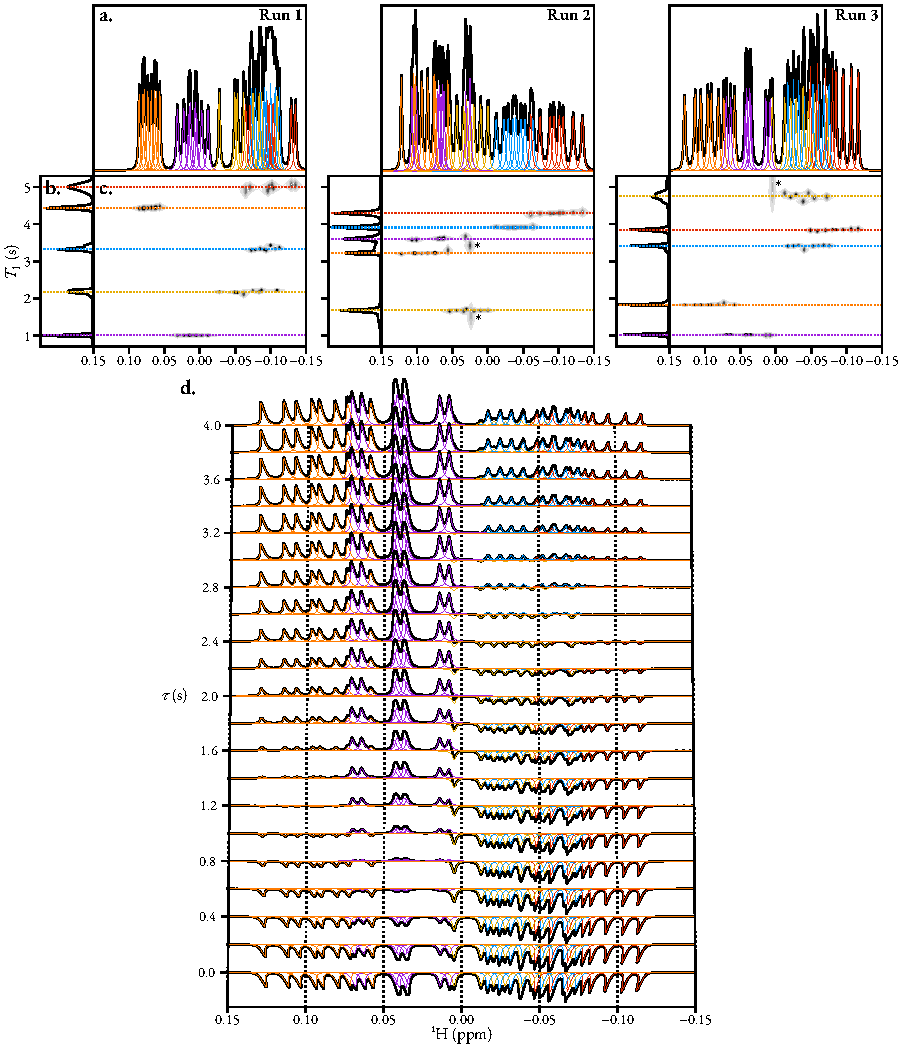
\includegraphics{five_multiplets_invrec/five_multiplets_invrec.pdf}
    \caption[
        Three examples of results generated wehn considering simulated
        inversion recovery datasets comprising five ddd multiplet structures.
    ]
    {
        Three examples of results generated when considering
        simulated inversion recovery datasets comprising five ddd multiplet
        structures.
        \textbf{a.} Plot of the result generated for the first increment ($\tau
        = \qty{0}{\second}$), with all the plots multiplied by $-1$. Black:
        spectrum of the data. Coloured lines: peaks corresponding to
        oscillators in the estimated model. Oscillators with the same colour
        are components of the same multiplet.
        \textbf{b.} Distribution of $T_1$ values, generated using
        \cref{eq:distribution}, with
        $p_{\text{min}} = \qty{0.7}{\second}$,
        $p_{\text{max}} = \qty{5.3}{\second}$,
        $c = 40$,
        $R=128$.
        \textbf{c.} \ac{DOSY}-style representation of the result, generated using
        \cref{eq:dosy-cross-product}.
        Dashed horizontal lines denote the true $T_1$ values for each spin.
        \textbf{d.} Estimation result for each increment for Run 3,
        illustrating the evolution of the amplitudes of each oscillator with
        $\tau$.
    }
    \label{fig:five-multiplets-invrec}
\end{figure}
\Cref{fig:five-multiplets-invrec} shows the result achieved by applying the
described method in determining the $T_1$ associated with signals in a set of
three of simulated inversion recovery datasets featuring 5 overlapping ddd
multiplet structures.
Each dataset was generated using spin systems such that within a
known region of the spectrum (\SIrange{0.15}{-0.15}{\partspermillion}) five ddd
multiplet structures with significant overlap, abiding by the weak coupling
approximation, were present.
Constraints were placed on the shifts and
couplings of the spin system to ensure that no two signals would have
frequencies with a difference less than $\nicefrac{\fswone}{\None}$.
For each spin, a $T_1$ value was sampled from $\mathcal{U}(\qty{1}{\second},
\qty{5}{\second})$, and a $T_2$ value was sampled from
$\mathcal{U}(\qty{0.2}{\second}, \qty{0.6}{\second})$.
The inversion recovery experiment was simulated using \textsc{Spinach}, with the
relaxation phenomena described by the ``extended $T_1$/$T_2$
approximation''\cite{SpinachRelax} (see also \cref{subsec:invrec-datasets}).
Each dataset was corrupted by \ac{AWGN} with a target \ac{SNR} of
\qty{40}{\deci\bel}.
The estimation routine outlined by \cref{alg:estimate-seq} was applied
to the generate a parameter estimate of the region of interest.

Despite heavy overlap between peaks, the routine was successful at
assigning each signal in the dataset with a $T_1$ value that closely agreed
with the $T_1$ of the spin giving rise to it (see
\cref{fig:five-multiplets-invrec}.b). As is to be
expected, in scenarios where little overlap existed between signals with
different decay rates, $T_1$ predictions tended to be more accurate, with
smaller associated errors (see for example the purple and orange multiplets in Run 1.
Nevertheless, adequate estimates could still be obtained in cases of severe
overlap (see the red, blue and yellow multiplets in Run 1). Particular
oscillators for which the estimate of $T_1$ is notably far from the true
value tended to be associated with large errors, with examples denoted with an
asterisk in \cref{fig:five-multiplets-invrec}.c.

\subsubsection{Andrographolide Diffusion}
\begin{sidewaysfigure}
    \centering
    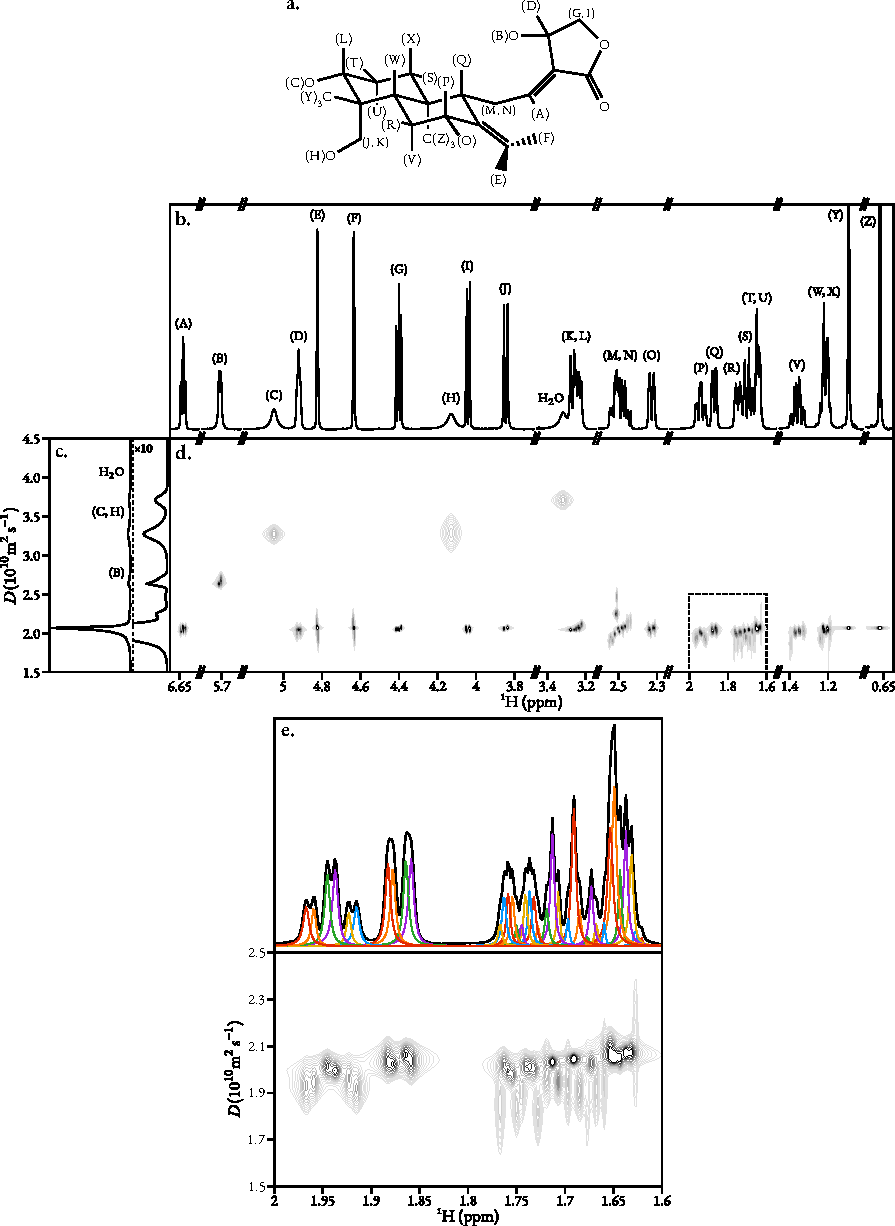
\includegraphics{andrographolide_dosy/andrographolide_dosy.pdf}
    \caption[
        The result of estimating a diffusion dataset of andrographolide.
    ]{
        The result of estimating a diffusion dataset of andrographolide in
        unfresh \acs{DMSOd6}.
        \textbf{a.} \ac{1D} spectrum.
        \textbf{b.} Diffusion profile obtained by projecting the contour plot in
        c onto the $y$-axis.
        \textbf{c.} Contour plot mapping estimated oscillators to diffusion constants, with
        $p_{\text{min}} = \qty{1.5e-10}{\meter\squared\per\second}$,
        $p_{\text{max}} = \qty{4.5e-10}{\meter\squared\per\second}$,
        $c = 2.5$,
        $R=128$.
        \textbf{d.} Magnified view of the \SIrange{2}{1.6}{\partspermillion}
        spectral range, with estimated oscillator peaks plotted.
    }
    \label{fig:andrographolide-dosy}
\end{sidewaysfigure}
\Cref{fig:andrographolide-dosy} shows the result of applying the
estimation technique on a oneshot \ac{DOSY} dataset of andrographolide in
unfresh \acs{DMSOd6} at \qty{298}{\kelvin}. Exposure of the sample to water is
evidenced by the broad
peak around \qty{3.3}{\partspermillion}, estimated to have a diffusion constant
of \qty{3.7e-10}{\meter\squared\per\second}. On top of this, the acidic
hydroxyl protons (B, C, H) of andrographolide show significant line-broadening,
and their estimated diffusion coefficients are considerably different compared
with those of the non-hydroxyl protons, due chemical exchange with water in the
sample\cite{Chen1998}.
The diffusion profile generated suggests a diffusion constant of andrographolide of
\qty{2.07e-10}{\meter\squared\per\second}. The predicted diffusion constant for
each estimated oscillator, especially those with greater intensity, shows
decent consistency.
Lower intensity oscillators, especially those which
significantly overlap with others, tended to be associated with
less consistent diffusion constants and larger errors with examples of this
phenomenon apparent in \cref{fig:andrographolide-dosy}.d of the figure. A few
oscillators also show a
significant deviation at around \qty{2.5}{\partspermillion}. This is due to the
presence of a 1:2:3:2:1 quintet from partially protonated \acs{DMSO}\footnote{
    This multiplet structure arises from the \ch{^1H} in \acs{DMSO} coupling to
    two
    equivalent spin-$1$ \ch{^2H} nuclei. The relative amplitudes of the signals
    can be deduced by considering the ``trinomial triangle'', an extension of
    the more familiar Pascal's triangle, the latter being applicable to
    couplings involving equivalent spin-$\nicefrac{1}{2}$ nuclei.
}. As the
data is insufficiently resolved to enable the separation of andrographoilde and
\acs{DMSO} signals, oscillators exist which have amplitude profiles
influenced by both species, leading to an aggregated diffusion constant. As
$D_{\text{DMSO}} > D_{\text{andrographoilide}}$, the affected oscillators
possess larger predicted diffusion constants.

\subsubsection{Glucose/Valine/Threonine Diffusion}
\begin{figure}
    \centering
    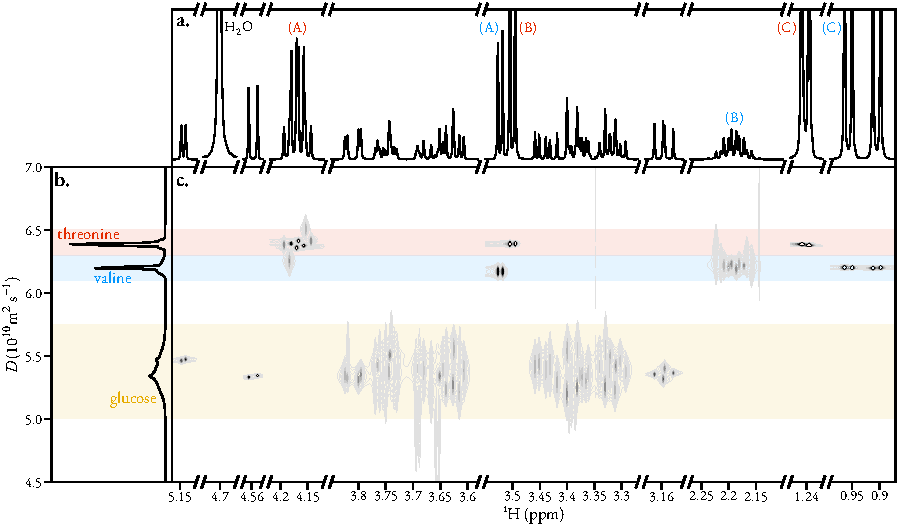
\includegraphics{glu_thre_val_diffusion/glu_thre_val_diffusion.pdf}
    \caption[
        The result of estimating a diffusion dataset for a mixture of L-threonine,
        L-valine and D-(+)-glucose.
    ]{
        The result of estimating a diffusion dataset for a mixture of L-threonine,
        L-valine and D-(+)-glucose in D\textsubscript{2}O.
        \textbf{a.} \acs{1D} spectrum, taken from the first \acs{FID} of the
        diffusion dataset.
        \textbf{b.} Diffusion coefficient distribution.
        \textbf{c.} \acs{DOSY}-style plot of chemical shifts vs diffusion
        constant, generated using \cref{eq:distribution}, with
        $p_{\text{min}} = \qty{4.5e-10}{\meter\squared\per\second}$,
        $p_{\text{max}} = \qty{7e-10}{\meter\squared\per\second}$,
        $R=256$, and $c=1.5$.
    }
    \label{fig:gluc_val_thre}
\end{figure}
Another diffusion example is provided by \cref{fig:gluc_val_thre}, where the
estimation routine was applied to a dataset derived from a sample comprising
the molecules L-valine ($M_r = \qty{117.148}{\gram\per\mole}$,
\cref{fig:structures}.c), L-threonine
($M_r = \qty{119.120}{\gram\per\mole}$, \cref{fig:structures}.d), and D-(+)-glucose ($M_r =
\qty{180.156}{\gram\per\mole}$, \cref{fig:structures}.e) dissolved in
D\textsubscript{2}O at \qty{298}{\kelvin}. Not included in the figure is the
result for the water signal, for which a diffusion constant of
\qty{1.88e-9}{\meter\squared\per\second} was determined. The routine
achieved decent separation of the three species in the sample. Predicted
diffusion coefficients for valine and threonine were
\qty{6.20e-10}{\meter\squared\per\second} and
\qty{6.39e-10}{\meter\squared\per\second}, respectively. For glucose, the situation is
complicated by the presence of two major anomeric forms:
\textalpha-D-glucopyroanose and
\textbeta-D-glucopyroanose\footnote{
    The equilibrium mixture in water comprises 38\% of the \textalpha\ isomer
    and 62\% of the \textbeta\ isomer.
    This is evidenced by the
    spectrum in \cref{fig:gluc_val_thre}.a, where the relative integrals of
    the doublets at \qty{5.15}{\partspermillion} and
    \qty{4.56}{\partspermillion} agree with this ratio.
    A tiny amount of the open-chain form will
    also be present, though in a negligible quantity.
}\cite[Chapter 3]{Davis2002}.
There is some evidence of separation of these anomers, principally due
to the downfield doublets at \qty{5.15}{\partspermillion} (\textalpha) and
\qty{4.56}{\partspermillion} (\textbeta), which have estimated diffusion
coefficients of \qty{5.47e-10}{\meter\squared\per\second}
and \qty{5.34e-10}{\meter\squared\per\second}, respectively. Beyond these
however, the other estimated oscillators corresponding to glucose have
associated errors which are too large for clear resolution of the two species.

As is to be expected, signals which are of greater intensity, and which are
more clearly resolved enable the determination of diffusion coefficients with
lower errors. A clear example of this behaviour can be recognised when
considering the valine result (see the area shaded blue in
\cref{fig:gluc_val_thre}.c). The
oscillators which lead to diffusion constants with the lowest errors correspond to
the high intensity doublet of doublets around \qty{0.95}{\partspermillion},
resulting from six equivalent protons from two methyl groups. Far
greater uncertainty is observed for the predictions associated with proton (B),
which has a doublet of septets structure, featuring many low-intensity signals.
Application of multivariate methods on the dataset was unsuccessful at
extracting diffusion information for the separate components. Both
\ac{DECRA} and \ac{SCORE} could extract the water
signal from the rest of the dataset, with the two components having associated
diffusion coefficients of \qty{6.31e-10}{\meter\squared\per\second}
and \qty{1.88e-9}{\meter\squared\per\second}, respectively.
